%%%%%%%%%%%%%%%%%%%%%%%%%%%%%%%%%%%%%%%%%%%%%%%%%%%%%%%%%%%%%%%%%%%%%%%
% Example Ansys Beamer Template
%%%%%%%%%%%%%%%%%%%%%%%%%%%%%%%%%%%%%%%%%%%%%%%%%%%%%%%%%%%%%%%%%%%%%%%
\documentclass[t]{beamer}

\usetheme{Ansys2024}

\usepackage{minted}
\usepackage{xcolor}
\usepackage{pdfpages}
\usepackage{listings}
\usepackage{tikz}
\usepackage{hyperref}

\usepackage[edges]{forest}
\hypersetup{
	colorlinks=true,
	linkcolor=blue,
	filecolor=magenta,      
	urlcolor=cyan,
}


\urlstyle{same}
\setbeamercolor{background canvas}{bg=}

\definecolor{bleudefrance}{rgb}{0.19, 0.55, 0.91}

%%%%%%%%%%%%%%%%%%%%%%%%%%%%%%%%%%%%%%%%%%%%%%%%%%%%%%%%%%%%%%%%%%%%%%%%%%%%%%%
\usetikzlibrary{shapes.geometric, arrows,positioning}

\tikzset{
	startstop/.style={
		rectangle, 
		rounded corners,
		minimum width=3cm,
		minimum height=0.75cm,
		align=center, 
		draw=black, 
		fill=ANSYS@Gold,
	},
	process/.style={
		rectangle, 
		minimum width=3cm, 
		minimum height=0.75cm, 
		align=center, 
		draw=black, 
		fill=ANSYS@Blue,
		text=white,
	},
	decision/.style={
		diamond, 
		aspect=4,
		minimum width=3cm, 
		minimum height=1cm,
		align=center,
		draw=black, 
		fill=ANSYS@Blue,
		text=white,
	},
	arrow/.style={thick,->,>=stealth},
	dec/.style={
		ellipse, 
		align=center, 
		draw=black, 
		fill=ANSYS@Bronze,
	},
}


\begin{document}
	
	%%%%%%%%%%%%%%%%%%%%%%%%%%%%%%%%%%%%%%%%%%%%%%%%%%%%%%%%%%%%%%%%%%%%%%%%%%%%%%%
	%% Title Slide
	
	\title{Ansys Python Manager}
	\subtitle{PyCon India 2024}
	%\author{Author: Abhishek Laxmikant Chitwar}
	\date{\today}
	\titleframe
	%%%%%%%%%%%%%%%%%%%%%%%%%%%%%%%%%%%%%%%%%%%%%%%%%%%%%%%%%%%%%%%%%%%%%%%%%%%%%%%
	%% Table of contents
	
	\begin{frame}{Table of Contents}
		\tableofcontents
		\vspace{200pt}  %% force top left  
	\end{frame}
	%%%%%%%%%%%%%%%%%%%%%%%%%%%%%%%%%%%%%%%%%%%%%%%%%%%%%%%%%%%%%%%%%%%%%%%%%%%%%%%
	%% What is Ansys Python Manager?
	
	%%%%%%%%%%%%%%%%%%%%%%%%%%%%%%%%%%%%%%%%%%%%%%%%%%%%%%%%%%%%%%%%%%%%%%%%%%%%%%%
	\subsection{What is Ansys Python Manager?}
	\begin{frame}
		\frametitle{What is Ansys Python Manager?}
		\vspace{-9pt}
		\begin{center}
			\begin{columns}[T]
				\begin{column}{.5\textwidth}
					\vspace{20pt} % Add some vertical space here  
					\small
					\begin{itemize}
						\item Collaborative open-source Python QT app.
						\item Developed by Ansys for beginner \& intermediate Python users.\\
						\vspace{5pt}
						\item Key Features
						\begin{itemize}
							\item Streamlines Python usage.
							\item Simplifies virtual environment management.
							\item Facilitates PyAnsys (open-source) package administration, easy access to documentation.
							\item Support for Windows \& Linux.
						\end{itemize}
					\end{itemize}
					\vspace{2pt}
				\end{column}
				\begin{column}{.5\textwidth}
					%% \vspace{-25pt}
					\centering
					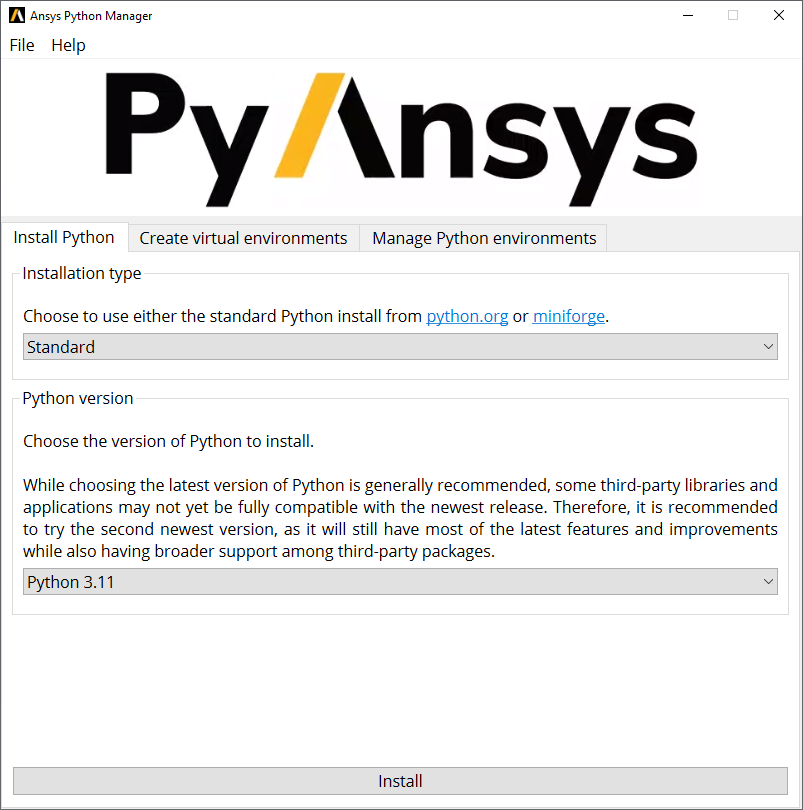
\includegraphics[width=0.9\textwidth]{assets/ansys_python_manager_screen_1.png}
				\end{column}
			\end{columns}
		\end{center}
		
	\end{frame}
	
	%%%%%%%%%%%%%%%%%%%%%%%%%%%%%%%%%%%%%%%%%%%%%%%%%%%%%%%%%%%%%%%%%%%%%%%%%%%%%%%
	%% Necessity for solution
	
	%%%%%%%%%%%%%%%%%%%%%%%%%%%%%%%%%%%%%%%%%%%%%%%%%%%%%%%%%%%%%%%%%%%%%%%%%%%%%%%
	\subsection{Necessity for solution}
	\begin{frame}
		\frametitle{Necessity for solution}
		\vspace{-9pt}
		\begin{center}
			\vspace{20pt} % Add some vertical space here  
			\small
			\begin{itemize}
				\item Transition Challenges
				\begin{itemize}
					\item Commercialization of famous Python management tools are roadblock for community.
				\end{itemize}
			\end{itemize}
			\vspace{2pt}
			\begin{itemize}
				\item Based on the internal scientific/engineering community response
				\begin{itemize}
					\item Developed the simplified solution.
					\item Focus on beginner and intermediate Python users.
					\item Provide a more accessible, user-friendly experience.
				\end{itemize}
			\end{itemize}
		\end{center}
	\end{frame}
	
	%%%%%%%%%%%%%%%%%%%%%%%%%%%%%%%%%%%%%%%%%%%%%%%%%%%%%%%%%%%%%%%%%%%%%%%%%%%%%%%
	%% Introduction to Ansys Python Manager
	
	%%%%%%%%%%%%%%%%%%%%%%%%%%%%%%%%%%%%%%%%%%%%%%%%%%%%%%%%%%%%%%%%%%%%%%%%%%%%%%%
	
	\subsection{Introduction to Ansys Python Manager}
	\begin{frame}
		\frametitle{Introduction to Ansys Python Manager}
		\vspace{-9pt}
		\begin{center}
			\begin{columns}[T]
				\begin{column}{.5\textwidth}
					\vspace{20pt} % Add some vertical space here  
					\small
					One stop shop for
					\begin{noitemize}
						\item
						\begin{minipage}{0.1\textwidth}
							
\includegraphics[width=0.5\linewidth]{0_smiley.png}
						\end{minipage}
						\hspace{-0.06\textwidth}
						\begin{minipage}{0.8\textwidth}
							Getting started with Python
						\end{minipage}
						\item
						\begin{minipage}{0.1\textwidth}
							
\includegraphics[width=0.5\linewidth]{1_smiley.png}
						\end{minipage}
						\hspace{-0.06\textwidth}
						\begin{minipage}{0.8\textwidth}
							Install Python
						\end{minipage}
						\item
						\begin{minipage}{0.1\textwidth}
							
\includegraphics[width=0.5\linewidth]{2_smiley.png}
						\end{minipage}
						\hspace{-0.06\textwidth}
						\begin{minipage}{0.8\textwidth}
							Create Virtual Environment
						\end{minipage}
						\item
						\begin{minipage}{0.1\textwidth}
							
\includegraphics[width=0.5\linewidth]{3_smiley.png}
						\end{minipage}
						\hspace{-0.06\textwidth}
						\begin{minipage}{0.8\textwidth}
							Manage Virtual Environments
						\end{minipage}
					\end{noitemize}
					\begin{itemize}
						\item Launching options
						\begin{itemize}
							\item Console
							\item JupyterLab
							\item Jupyter Notebook
							\item Spyder
							\item VS Code
						\end{itemize}
					\end{itemize}
				\end{column}
				\begin{column}{.5\textwidth}
					%% \vspace{-25pt}
					\centering
					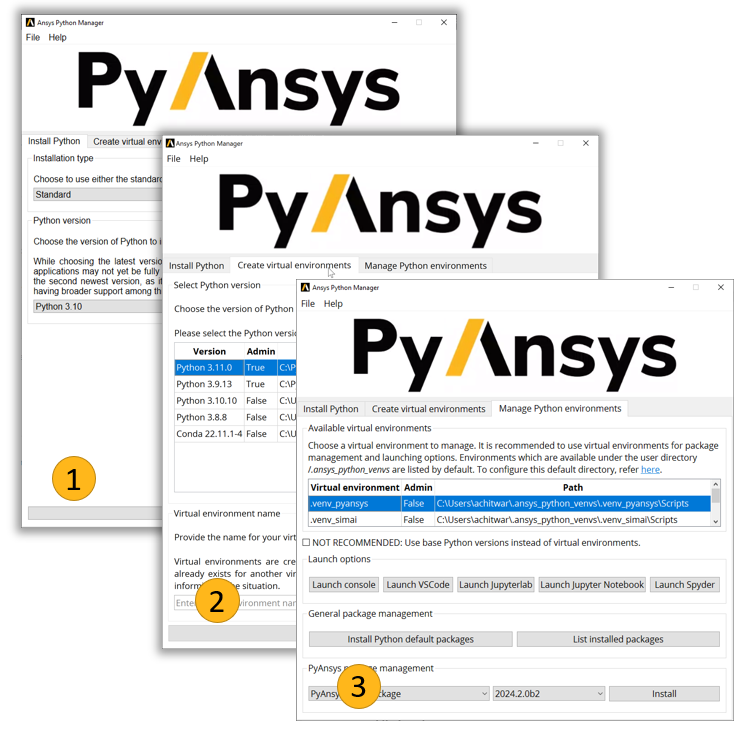
\includegraphics[width=0.9\textwidth]{assets/ansys_python_manager_screen_2.png}
				\end{column}
			\end{columns}
		\end{center}
	\end{frame}
	
	
	%%%%%%%%%%%%%%%%%%%%%%%%%%%%%%%%%%%%%%%%%%%%%%%%%%%%%%%%%%%%%%%%%%%%%%%%%%%%%%%
	%% Live Demo & Tips & Tricks
	
	%%%%%%%%%%%%%%%%%%%%%%%%%%%%%%%%%%%%%%%%%%%%%%%%%%%%%%%%%%%%%%%%%%%%%%%%%%%%%%%
	
	\subsection{Live Demo \& Tips \& Tricks}
	\begin{frame}[fragile]
		\frametitle{}
		\vspace{60pt}
		\begin{center}
			Live Demo \& Tips \& Tricks
		\end{center}
		\vspace{70pt}
		\tiny
		\begin{noitemize}
			\setlength\itemsep{0pt} % Adjust the vertical space between items  
			\item \textbf{License:} Ansys Python Manager is licensed under the MIT license. No commercial claim over Ansys whatsoever. For further licensing information refer \href{https://github.com/ansys/python-installer-qt-gui?tab=License-1-ov-file#readme}{here}.
			\item \textbf{Distributing:} This project is vectored to be an open-source project. For the time being, feel free to distribute it internally, but direct users to visit the \href{https://github.com/ansys/python-installer-qt-gui/releases}{Releases} page.
			\item \textbf{Security:} The versions that are still supported for security updates can be found at the \href{https://github.com/ansys/python-installer-qt-gui/blob/main/SECURITY.md}{Security guidelines} site. Information on how to report vulnerabilities is also found.
		\end{noitemize}
	\end{frame}
	
	%%%%%%%%%%%%%%%%%%%%%%%%%%%%%%%%%%%%%%%%%%%%%%%%%%%%%%%%%%%%%%%%%%%%%%%%%%%%%%%
	
	\lastframe{}
	
\end{document}